\documentclass{article}


\usepackage[english]{babel}
\usepackage[utf8]{inputenc}
\usepackage{amsmath}
\usepackage{graphicx}
\usepackage{subfigure}
\usepackage{hyperref}
\usepackage{listings}
%\usepackage{} adicionar as packages necessárias para os documentos.

\usepackage{color}

\definecolor{codegreen}{rgb}{0,0.6,0}
\definecolor{codegray}{rgb}{0.5,0.5,0.5}
\definecolor{backcolour}{rgb}{0.95,0.95,0.92}

\lstdefinestyle{codestyle}{
	basicstyle=\ttfamily,
    keywordstyle=\color{blue}\ttfamily,
    stringstyle=\color{red}\ttfamily,
    commentstyle=\color{magenta}\ttfamily,
    morecomment=[l][\color{codegreen}]{\#},
    backgroundcolor=\color{backcolour},
    breakatwhitespace=false,
    breaklines=true,
    captionpos=b,
    keepspaces=true,
    numbers=left,
    numbersep=5pt,
    showspaces=false,
    showstringspaces=false,
    showtabs=false,
    tabsize=2
}

%%%%%%%%%%%%%%%%%%%%%%%%%%%%%%%%%%%%%% INICIO %%%%%%%%%%%%%%%%%%%%%%%%%%%%%%%%%%%%
\title{Workshop \LaTeX - Template} %cmudar o título para o vosso Workshop
\author{Diogo Martins} % mudar o vosso nome dentro do {}
\date{\today} %mudar para a data de hoje. A função \today atualiza sempre para o dia em que se utiliza o documento
%%%%%%%%%%%%%%%%%%%%%%%%%%%%%%%%%%%%%%%%%%%%%%%%%%%%%%%%%%%%%%%%%%%%%%%%%%%%%%%%%%



%%%%%%%%%%%%%%%%%%%%%%%%%%%%%%%%%%%%%% DOCUMENTO %%%%%%%%%%%%%%%%%%%%%%%%%%%%%%%%%
\begin{document}

\maketitle %adiciona o título, autor, etc

\begin{abstract}
In the abstract, one should explain very briefly the content of the paper.
\end{abstract}


\tableofcontents %adiciona o índice
\newpage %nova página. Empurra tudo para a página seguinte.

\section{Introduction}

\subsection{What is \LaTeX?}
LATEX (pronounced LAY-tek or LAH-tek) is a tool used to create professional-looking  documents. It is based on the WYSIWYM (what you see is what you mean) idea, meaning you only have focus on the contents of your document and the computer will take care of the formatting. Instead of spacing out text on a page to control formatting, as with Microsoft Word or LibreOffice Writer, users can enter plain text and let LATEX take care of the rest.


\subsection{Why Learn \LaTeX?}
LATEX is used all over the world for scientific documents, books, as well as many other forms of publishing. Not only can it create beautifully typeset documents, but it allows users to very quickly tackle the more complicated parts of typesetting, such as inputting mathematics, creating tables of contents, referencing and creating bibliographies, and having a consistent layout across all sections. Due to the huge number of open source packages available (more on this later), the possibilities with LATEX are endless. These packages allow users to do even more with LATEX, such as add footnotes, draw schematics, create tables etc.

One of the most important reasons people use LATEX is that it separates the content of the document from the style. This means that once you have written the content of your document, we can change its appearance with ease. Similarly, you can create one style of document which can be used to standardise the appearance of many different documents. This allows scientific journals to create templates for submissions. These templates have a pre-made layout meaning that only the content needs to be added. In fact there are hundreds of templates available for everything from CVs to slideshows.
\subsection{What can I do with it?}
\begin{itemize}
    \item Documents;
    \begin{itemize}
        \item Reports;
        \item Thesis;
        \item Papers;
        \item Dissertations;
        \item Many others!
    \end{itemize}
    \item Presentations;
    \item Curriculum Vitae;
    \item Formal Letters;
    \item Newsletters;


\end{itemize}


\subsection{Software}
\begin{figure}[h!]
\centering
\subfigure[]{
\includegraphics[width=0.3\textwidth]{Image/overleaf.png}} 
\subfigure[]{
\includegraphics[width=0.3\textwidth]{Image/sharelatex.png}} 
\subfigure[]{
\includegraphics[width=0.3\textwidth]{Image/miketex.png}} 
\caption{(a) Overleaf (b) ShareLaTeX (c) MikTeX}
\end{figure}


\newpage    

\section{Writing with\LaTeX} \label{sec:examples}

Your introduction goes here! Some examples of commonly used commands and features are listed below, to help you get started.



\subsection{How to Include Figures}

Use the includegraphics command to include images. Use the figure environment and the caption command to add a number and a caption to your figure.

\begin{figure}[ht]
  \centering
  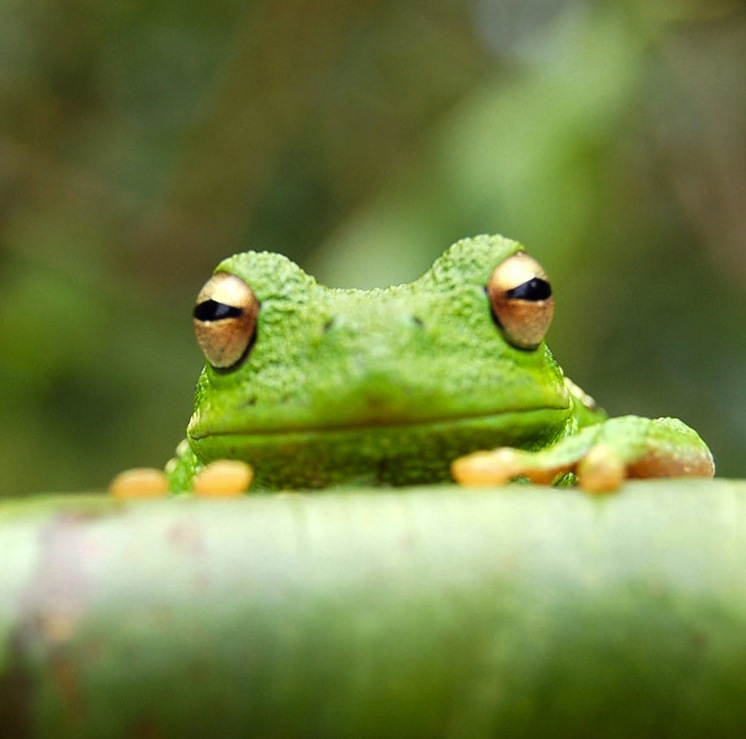
\includegraphics[width=1\textwidth]{Image/frog.jpg}
  \caption{These gloves are made of \LaTeX{}}
  \label{fig:latex}
\end{figure}

\begin{figure}[ht]
    \centering
    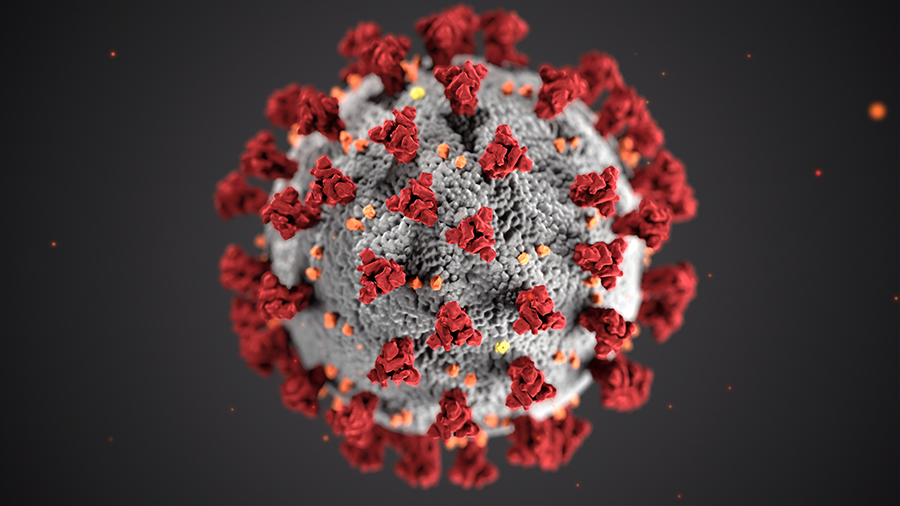
\includegraphics[width=0.75\textwidth]{Image/covid19.jpg}
    \caption{Corona Virus}
    \label{fig:covid}
\end{figure}

So if I remember correctly, figure~\ref{fig:covid} is \LaTeX{}.

\subsection{How to Make Tables}

Use the table and tabular commands for basic tables --- see Table~\ref{tab:widgets}, for example.

\begin{table}[ht]
\centering
\begin{tabular}{l|r}
  Item & Quantity \\ \hline
  Widgets & 42 \\
  Gadgets & 13
\end{tabular}
\caption{\label{tab:widgets}An example table.}
\end{table}

\subsection{How to Make Sections and Subsections}

Use section and subsection commands to organize your document. \LaTeX{} handles all the formatting and numbering automatically. Use ref and label commands for cross-references.

\subsection{How to Make Lists}

You can make lists with automatic numbering \dots

\begin{enumerate}
\item Like this,
\item and like this.
\end{enumerate}
\dots or bullet points \dots
\begin{itemize}
\item Like this,
\item and like this.
\end{itemize}
\dots or with words and descriptions \dots
\begin{description}
\item[Word] Definition
\item[Concept] Explanation
\item[Idea] Text
\end{description}

\subsection{How to Write Mathematics}

\LaTeX{} is great at typesetting mathematics. Let $X_1, X_2, \ldots, X_n$ be a sequence of independent and identically distributed random variables with
$\text{E}[X_i] = \mu$ and $\text{Var}[X_i] = \sigma^2 < \infty$, and let
$$S_n = \frac{X_1 + X_2 + \cdots + X_n}{n}
      = \frac{1}{n}\sum_{i}^{n} X_i$$

denote their mean. Then as $n$ approaches infinity, the random variables $\sqrt{n}(S_n - \mu)$ converge in distribution to a normal $\mathcal{N}(0, \sigma^2)$.

Instead of it you can create a equation.
\begin{equation}
    S_n = \frac{X_1 + X_2 + \cdots + X_n}{n} = \frac{1}{n}\sum_{i}^{n} X_i
\end{equation}

\subsection{How to add Citations and a References List}

You can upload a \verb|.bib| file containing your BibTeX entries, created with JabRef; or import your \href{https://www.overleaf.com/blog/184}{Mendeley}, CiteULike or Zotero library as a \verb|.bib| file. You can then cite entries from it, like this: \cite{WorkshopLaTeX}. Just remember to specify a bibliography style, as well as the filename of the \verb|.bib|.



\subsection{Code Snippets}
\lstinputlisting[language=C++, style=codestyle, showstringspaces=false]{hello.cpp}

\newpage
\section{Conclusions}

Everybody loves conclusions.

\newpage
\bibliographystyle{alpha}
\bibliography{sample}


\end{document}
